\begin{frame}{Can we automate performance debugging for distributed systems?}
  %%
  %% The columns environment is provided by beamer,
  %% see "texdoc beamer", Sec. 12.7 'Splitting a Frame into Multiple Columns'
  %%
  %% parameter: c - center columns vertically
  %%            t - align columns on the baseline of the first line
  %%                don't use, if a column contains (only) a graphic!
  %%            T - align columns on the top of the first line (ok with graphics)
  %%            b - align columns on the bottom line
  \begin{columns}[T]
    %% Each column must be given a with.
    %% Should be given relative to \textwidth:
    \begin{column}{.55\textwidth}
      {
      \small
      \begin{itemize}
        \item A distributed system is comprised of various components (fig 1).
        \item When debugging a problem, it is often hard to pinpoint the \textit{exact}
        problematic area.
          \item Software developers have to \textit{manually} and \textit{repeatedly} instrument the codebase or
          enable more logging.
        \item Use ``signals'' as feedback in a loop to automate the ``zoom in'' process (fig 2).
      \end{itemize}
      }
    \end{column}
    \begin{column}{.4\textwidth}
      %% here, \textwidth is the with of the current column

      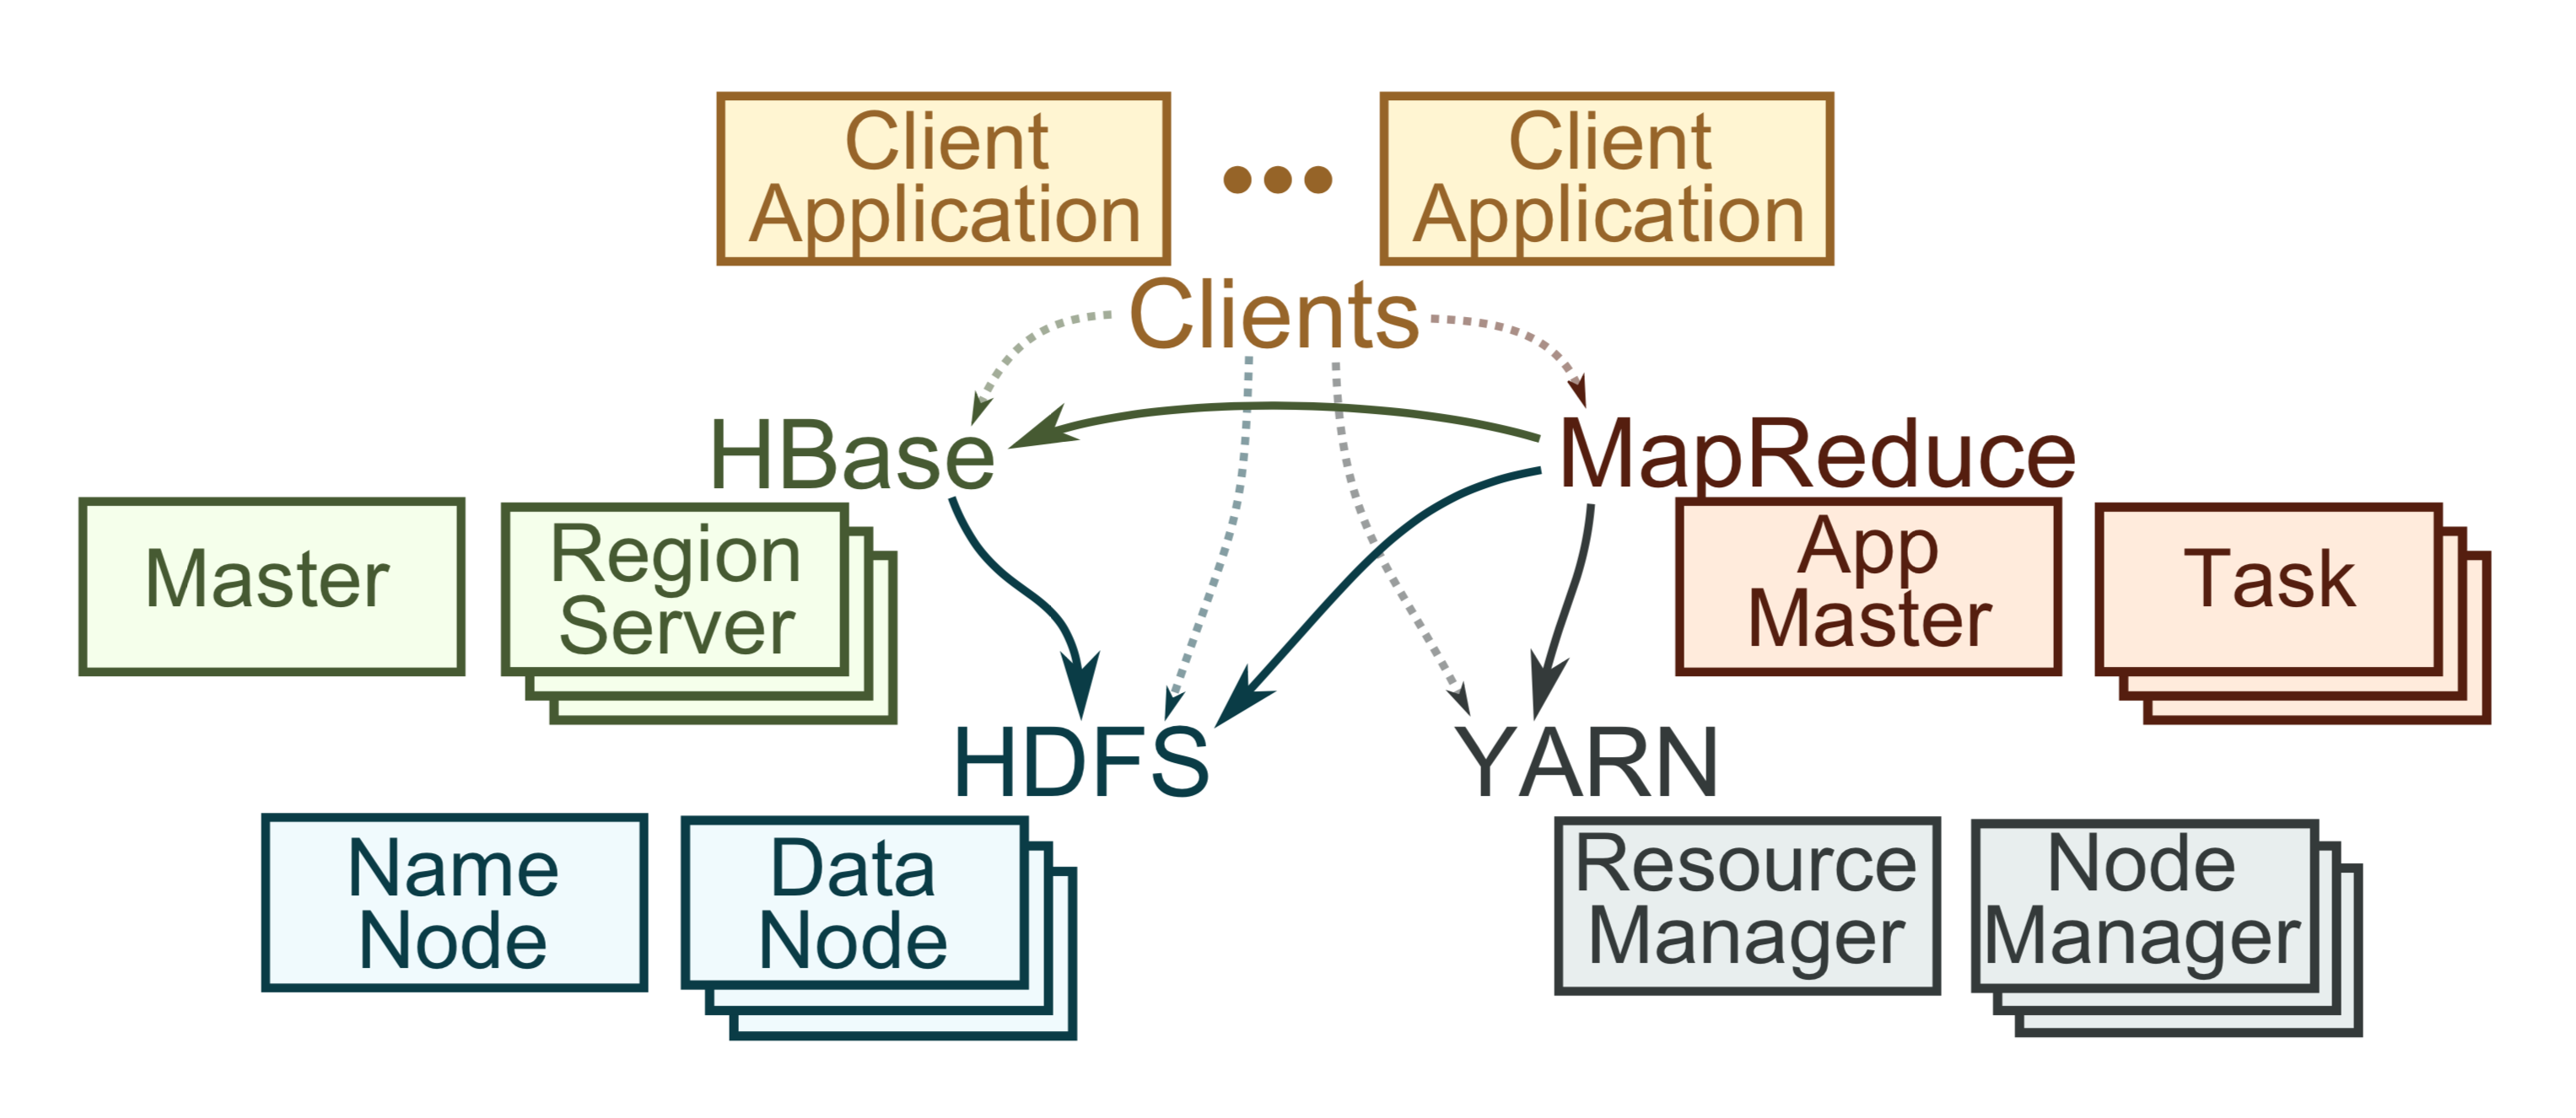
\includegraphics[width=.9\textwidth]{figures/dist-sys.png}

      {\tiny Fig 1: Components in Hadoop. }
      % \\Each system comprises several processes on potentially many machines.}

      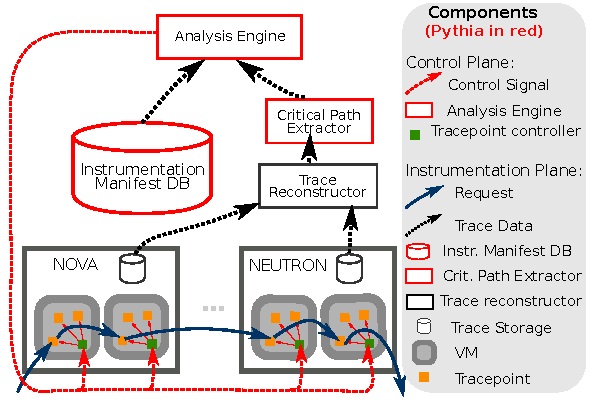
\includegraphics[width=.9\textwidth]{figures/architecture.pdf}

      {\tiny Fig 2: Arch. of a just-in-time instrumentation framework.}

    \end{column}
  \end{columns}
\end{frame}


